\cotefile{87}
\scanpage{15}
% L1–3. Vertical rule at the left of the assertion.
\uline{Cor. 6} Soit $F\in\mathrm{Fac}(C)$ ($C$ polyèdre convexe)
Alors pour tt $-1\leq i\leq d=\dim F$, existe $F'\leq F$
telle que $\dim F'=i$.

% L4–9. Horizontal strokes at the two ends, oblique strokes across the block.
\deleted{Clair si $d=-1$ ou $0$, sinon. On \unsure{ad.|dit} qu'il
\inserted{\unsure{procède} par} récurrence sur $d$, clair si $d=-1,0$. Si $d\unsure{\geq|>}0$,
$\exists\ F'$ tel que $F'\ne\varnothing,F$\quad $\varnothing<F'<F$ (cor. 4)
Donc $\dim F'=d'<d$. Si $i\leq d'$ on gagne, par
hyp. de récurrence appliquée à $F'$. \unsure{Si}
Sinon on gagne par l'hyp. de récurrence.}

% L10–15
Formel à partir du cor. 5, qui implique que
si $x\unsure{\leq|<} y$, $x,y\in\mathrm{Fac}(C)$, \deleted{\unsure{alors}} $\exists$ chaîne
$x_0=x<x_1<\ldots x_n=y$, avec $x_{i+1}$ succ de $x_i$
$(0\leq i\leq n-1)$, et qu'alors \deleted{$d(y)-d(x)=n$.}
\deleted{$d\unsure{(x)|(}\quad d\unsure{(}$} $d(x_i)-d(x_0)=i$ i.e. $d(x_i)=d(x_0)+i$.
[On \unsure{prendra|prend} $y=F$, $x=\varnothing$ \ldots{} ]

% L16–20. Vertical rule at the left of the assertion.
\uline{Cor. 7} Soit $\unsure{P|\mathcal P|\Phi}$ un polyèdre combinatoire
strict, $d$ une fonction dimension sur $P$
(cf cor. 5) \unsure{Soient|Soit} $x,y\in P$, $x<y$,
$d(y)=d(x)+2$. Alors l'ens des $z\in P$,
tels que $x<z<y$ est de cardinal $2$.

% L21–24
$P_{x,y}$ est un polyèdre combinatoire \inserted{strict} de
dim $(-1)+2=1$, donc provient d'un polyèdre
convexe de dim $1$, i.e. d'un segment. Celui-ci a exactement $2$ extrémités !
% archive sheet number: 14

\scanpage{16}
% L1. Pencil count to the left of the ink title.
\margin{(\unsure{13 p|13 p.})} \hfill Cube
% archive sheet number: 15

\scanpage{18}
% L1–4
Caractérisation intrinsèque d'un $n$-cube, déterminé par un ens
\[
\unsure{P|\mathcal P|\Phi}\subset\mathrm{Espaff}(E)
\]
de sous-espaces affines d'un espace affine sur $\unsure{k|h}$ :

% L5–8
a) $P$ \deleted{a un plus petit et un plus grand élément, et}
\inserted{contient $\varnothing$ et $E$ (qui sont donc un plus petit et un plus grand élément), et}
dans $P^{\unsure{**|\times\times}}=P-\{0_P,1_P\}$ ($P$ privé de son plus
petit et plus grand élément) tout élément est
intersection \inserted{(pour la rel. d'ordre)} d'éléments maximaux.

% L9–14
b) Pour tt élément maximal $F$ de $P^{**}$, $\exists!$
él. maximal $F'$ tel que $\mathrm{Inf}_{P^{\deleted{\unsure{**}}}}(F,F')=\varnothing$ [i.e.
$(F,F')$ non minoré dans $P^{**}$ i.e. $F\cap F'$ ne contient
aucun él. de $P$ différent de $\varnothing$] [Ainsi l'ens
$B$ des él maximaux de $P^{**}$ est muni d'une involution $\sigma$ :
$F-F'$ ss pt fixe\unsure{.|..|\ldots{}}]

% L15–21
c) Si à tte $V\in P^{\deleted{\unsure{**}}}$, \inserted{$V\ne\varnothing$}, on associe l'ens \deleted{\unsure{$A$|$B$}} $B_V$
des $b\in B$ qui le majorent, on trouve
une partie \inserted{$A$} de $B$ telle que $b\in A\Longrightarrow\sigma b\notin A$
(i.e. une section partiellement définie de $B$
sur $I=B/\sigma$). Ceci posé, l'application
\[
P\setminus\{\varnothing\}\longrightarrow\Gamma_{\mathrm{part}}(B/I)
\]
ainsi définie, qui est injective par b), est bijective.

% L22–27
\margin{\uline{NB} a) b) c) signifient que l'ens ordonné $P$ est un cube combinatoire}
d) Si $n=\dim\,\mathrm{comb}\,P$, on a \deleted{$E$} $n=\deleted{\unsure{d}}\mathrm{rg}\ E
=\frac12\operatorname{card} B$.

[ a) à d) implique que \inserted{si $V\in P$, $\dim_P V=\dim_E V$, que}
le $\mathrm{Inf}$ \deleted{\unsure{dans $P$|dans $\Phi$}} \inserted{d'une}
partie minorée de $P\setminus\{0\}$ est aussi son
intersection (en tant qu'ens. de parties
de $E$) \inserted{et que les ``hyperplans'' \deleted{\unsure{$E$}} $\in P$ passant par un sommet $s\in P$ sont lin. indép.}. Mais celà n'implique pas que le
% archive sheet number: 17

\scanpage{19}
% L1–6. Continuation of the bracket opened on scan 18.
$\mathrm{Inf}$ d'une partie de $\unsure{P|\mathcal P|\Phi}$ (dans $P$) est $\varnothing$, i.e. si son
intersection ne contient pas d'él. de $P\setminus\{\varnothing\}$,
que cette intersection soit vide. Ex : \deleted{\unsure{un}} quadrilatère
qui n'est pas un parallélogramme
\figure{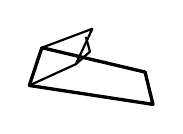
\begin{tikzpicture}[x=1cm,y=1cm,line cap=round,line join=round]
\draw[very thick] (0,0)--(.16,.48)--(1.47,.17)--(1.57,-.24)--cycle;
\draw[thick] (0,0)--(.59,.27)--(.8,.72)--(.16,.48);
\draw[thick] (.59,.27)--(.77,.43)--(.72,.61);
\end{tikzpicture}}.
L'axiome qui suit assure qu'il en est
pourtant ainsi\ldots{} ]

% L7–11
e) Si $b,b'$ sont des él. maximaux de $P$
\inserted{(i.e. $b,b'\in B$)} dont le $\inf$ est $\varnothing$ (i.e. $b'=\sigma b$), alors \deleted{\illegible{2}}
$b\cap b'=\varnothing$ (i.e., \deleted{\unsure{b,b'}} par d), \inserted{$b,b'$ sont \unsure{des|alors}}
\deleted{\unsure{2 à} des sous-variétés lin. parallèles}
hyperplans affines parallèles\ldots).

% L12–17
Dans l'espace des translations $T$ de $V$,
les \deleted{\unsure{des}} espaces directeurs $H_i$ $(i\in I)$ des
\deleted{\unsure{des}} deux \deleted{sous-espaces linéaires} \inserted{hyperplans affines} $b\in B$ sont
lin. indép, et correspondent donc à
une décomposition $\displaystyle T\simeq\prod T_i$ $(T_i=T/H_i)$
de $T$ en produit de droites. La donnée
% L18–24
du $T$-torseur $E$ revient à la donnée
d'une famille $(\deleted{T}E_i)_{i\in I}$ de $\deleted{\unsure{E}}T_i$-torseurs.
$E_i\simeq E/H_i$. De plus, dans chaque
$E_i$ il y a \inserted{une partie de} deux pts distincts, \deleted{\unsure{soit}} \unsure{q} $B_i$,
(isom. à la fibre de $B/I$ en $i\in I$). Or
on vérifie que la donnée \deleted{d'un} (pour $i$
% archive sheet number: 18

\scanpage{20}
% L1–4
fixé) d'un $T_i,E_i,B_i\subset E_i$ équivaut en fait
à la donnée de $B_i$ (comme torseur sous
$\pm1$ !) en prenant
\[
T_i=\mathrm{Ker}\,(k^{B_i}\overset{\varepsilon}{-}k),\quad E_i=\varepsilon^{-1}(1)
\]

% L5–10
Donc la donnée \deleted{des} \deleted{\unsure{de la}} \inserted{d'une} famille $(T_i,E_i,B_i)_{i\in I}$
\inserted{($\operatorname{Card} I=n$)} équivaut à
la donnée d'un \unsure{ens orienté|squelette|ens orient.} de $n$-cube.
Montrons que cette donnée permet de
reconstruire le $n$-cube, comme le
produit de la famille (indexée par $I$)
des $1$-cubes ---

% L11–14
On a aussi
\[
\begin{aligned}
T&=\mathrm{Ker}\,(k^B\overset{\overset{\nearrow\,\text{trace}}{\mathrm{tr}}}{-}k^I)\\
E&=\mathrm{tr}^{-1}(1)
\end{aligned}
\]
Si $J\subset I$, on considère
% archive sheet number: 19

\scanpage{22}
% L1–5
Soit $n$ un entier, $k$ un anneau \inserted{comm} avec $2$ inv. ds $k$
$C_n$ catégorie formée des
\[
\left\{\begin{aligned}
& k\text{-module }E\\
& \inserted{1}\ \deleted{\unsure{\text{famille}}}\,\text{famille }(E_i)_{i\in I}\ \text{de sous-modules libres de }E\\
& \forall i\in I,\ \text{partie } B_i\text{ de }E_i
\end{aligned}\right.
\]

% L6–9
avec axiomes
\[
\begin{aligned}
&\text{a) } E\text{ somme directe des } E_i\\
&\text{b) }\operatorname{card} B_i=2\qquad(\forall i\in I)\\
&\text{c) }\forall b\in B_i,\ \{b\}\text{ base de } E_i\\
&\text{d) }B_i=-B_i
\end{aligned}
\]

% L10–15
% slanted
\margin{épure \deleted{\unsure{combinatoire}} \deleted{\unsure{cubique}} de $n$-cube \deleted{\unsure{combinatoire}}}
$\mathcal D_n^{\unsure{*|+}}$ catégorie formée des ens $B$ de card. $2n$,
munis d'une relation d'équiv. $R$ à orbites
de cardinal $2$ (donc $B/R=I$ de card $n$)
-- ou encore des ens. de card $2n$, avec
\deleted{involution} \inserted{$\{\pm1\}$} opérant dessus librement i.e. avec une
involution sans pts fixes.

% L16–20
\[
 C_n\unsure{\longrightarrow|-}\mathcal D_n\qquad\text{par}\quad
 (E,(E_i)_{i\in I},(B_i)_{i\in I})\longmapsto\{\bigcup B_i,\ldots\}
\]
Mais on a aussi
\[
 \mathcal D_n\longrightarrow C_n\qquad\text{en posant}
\]
% The sequence at the left is circled.
\margin{\tikz[baseline=(q.base)]\node[draw,ellipse,inner sep=2pt](q){$\scriptstyle 0\longrightarrow E-k^B\longrightarrow k^I-0$};}
\[
 E=\coprod_{i\in I}B_i\wedge_{\{\pm1\}}k
\]
\margin{\uline{ou aussi} $E\subset k^{(B)}$ formé des $\sum_{b\in B}\lambda_b e_b$ avec $\lambda_{-b}=-\lambda_b$}
où $\{\pm1\}$ opère sur $k$ par homothéties. Donc les
deux catégories sont équivalentes.
% archive sheet number: 21

\scanpage{23}
% L1–3
En fait, le $E$ envisagé a \deleted{nécessairement} une
forme quadratique canonique, car chaque
$B_i\wedge_{\{\pm1\}} k$ a la forme \unsure{standard|standart|bilinéaire} \inserted{de produit scalaire} $(x,y)=xy$.

% L4–5
Je dis qu'on a un isom canonique
\[
\omega_E\simeq\omega_I\wedge\bigwedge_{i\in I}\deleted{\unsure{B_i}} B_i
\]

% L6–7
En effet, par la formule d'associativité on a
\[
\omega_E\simeq\omega_I\wedge\bigwedge_{i\in I}\omega_{E_i}
\]

% L8–9
et d'autre part
\[
\omega_{E_i}\simeq\deleted{\unsure{\omega_{B_i}|\omega_{E_i}}} B_i
\]

% L10–12
% slanted
\margin{faire tomber l'indice $i$}
[ On a en effet, comme $\deleted{\unsure{B}} B_i\subset$ ens des bases de $E_i$,
$B_i\longrightarrow\omega_{E_i}$, et on voit que c'est inj, donc
bijectif \ldots. ]

% L13–14, lower right
\uline{\deleted{Cube combinatoire}} \inserted{épure \deleted{de} $n$-cube}
\uline{orienté}
% Isolated diagonal pen stroke below the text.
\figure{\begin{tikzpicture}\draw (0,0)--(.86,-1.30);\end{tikzpicture}}
% archive sheet number: 22

\scanpage{24}
% L1–2
\uline{Polyèdre combinatoire} associé à un polyèdre convexe :
l'ens des facettes \inserted{$\ne$ l'unique facette maximale}, \deleted{\unsure{autre que}} ordonné par $\overline F\subset\overline{F'}$.

% L3–8
[ La dim d'une facette se retrouve sur le
polyèdre combinatoire comme une dim.
combinatoire (d'un él d'un ens. ordonné) :
sup des longueurs des chaînes ascendantes
$F_0\lneq F_1\lneq\ldots\lneq F_n=F$ -- ou longueur commune
des chaînes maximales \ldots{} ]

% L9–13
\[
\unsure{P|\mathcal P|\Phi}_0\quad P_1\quad\text{--}\quad
P_{n-1}\deleted{\unsure{\{C\}|[C]}}\qquad (n=\dim C)
\]
\unsure{où|Si} $P_i=$ ens des facettes de dim. $i$
Entre $P_i$ et $P_{i+1}$ $(0\leq i\leq n-1)$ relation d'incidence \inserted{$R_i$}.
La relation d'ordre sur $P\simeq\coprod_{0\leq i\leq n}P_i$ se
réconstitue à partir des $R_i$.

\begin{center}-- -- -- -- --\end{center}

% L14–20. Left vertical rule.
\uline{Proposition} Les facettes \inserted{$\ne\varnothing$} du \deleted{\unsure{$(B,R)$}} \inserted{cube $C(B,R)$} sont en
corr. biunivoque avec l'ens des \deleted{\unsure{f}} Sections
partielles de $B$ sur $I=B/R$. Si
\diagram{\begin{tikzcd}[ampersand replacement=\&,column sep=small]
\sigma\colon J\arrow[rr,bend right=17] \&[-1.4em] \subset I \& B
\end{tikzcd}}
est une telle section, la
facette \uline{fermée} \inserted{(ouverte)} associée est l'ens des
$\displaystyle\sum_{b\in B}\lambda_b.b$ avec $\lambda_{-b}=-\lambda_b$, $\lambda_{\sigma(\unsure{j|y})}=+1$, et
$|\lambda_b|\leq 1$ (resp $|\lambda_b|<1$) pour $b\in I\unsure{-|\setminus}J$.
% archive sheet number: 23

\scanpage{25}
% L1–3
Soient $\lambda=\sum_{b\in B}\lambda_b e_b$, $\mu=\sum_{b\in\unsure{B|D}}\mu_b e_b$ deux éléments de $C$
($\lambda_{-b}=-\lambda_b$, $|\lambda_b|\leq 1$, idem pour $\mu$) quand a-t-on
$R(\lambda,\mu)$ (relation d'équiv. des facettes ?)

% L4–10
Si $\lambda\ne\mu$, on veut que \deleted{\unsure{On}} $\exists\,t\in\mathbb R$, $t\lambda+(1-t)\mu\in C$,
avec au choix $t<0$, ou $t>1$. \deleted{\unsure{Pour le|Pour les}} On veut
\deleted{$t\lambda_b\unsure{+}$} donc $|t\lambda_b+(1-t)\mu_b|\leq1$. Si $\lambda_b=\mu_b$,
aucun Pb, si $|\lambda_b|,|\mu_b|<1$, non plus
le seul Pb si $\lambda_b\ne\mu_b$, et $\lambda_b\ \unsure{\underline{\text{ou}}|=}\ \mu_b=\pm1$
\figure{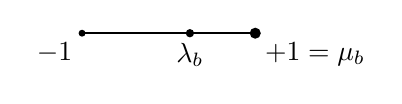
\begin{tikzpicture}[x=1cm,y=1cm]
\draw[thick](0,0)--(2.2,0);
\fill (0,0) circle (1.25pt) node[below left]{$-1$};
\fill (1.37,0) circle (1.5pt) node[below]{$\lambda_b$};
\fill (2.2,0) circle (2pt) node[below right]{$+1=\mu_b$};
\end{tikzpicture}}
Il faut donc
\[
\begin{aligned}
&|\lambda_b|=1\ \text{\uline{ou}}\ |\mu_b|=1\\
&\Longrightarrow\lambda_b=\mu_b\qquad\deleted{\unsure{\text{d}|\text{donc}}}
\end{aligned}
\]

% L11–14
Donc \deleted{a) L'ens \unsure{$J(\mu)$|$J(\lambda)$} des $\lambda$}

a) Soit $J(\lambda)=\{b\in B\mid\lambda_b\deleted{\unsure{\in}}=\pm1\}$. On veut $J(\lambda)=J(\mu)$ soit $J$

b) Si $j\in J$, on veut $\lambda_b=\mu_b$

La proposition s'ensuit.

% L15–18
\uline{Corollaire} La relation d'ordre entre facettes
de $C=C(B,R)$ est inverse de la relation de
prolongement entre sections partielles de
$B$ sur $I=B/R$.

% L19–24
La facette maximale correspond à la section
partielle vide ($J=\varnothing$). Les facettes sous-maximales correspondent aux éléments de $B$.
Deux facettes ss-maximales distinctes \inserted{\deleted{\unsure{se}} ne} se rencontrent
pas (``sont $//$'') ssi elles correspondent à des pts
$x,y$ de $B$ qui sont congrus par $R$.
% archive sheet number: 24

\scanpage{26}
% L1–4
\uline{Exercice} Soit $B\xrightarrow{p}I$ une application \inserted{\unsure{surjective|surjection}} \deleted{telle que
$\forall i\in I$, $\operatorname{card}p^{-1}(i)\geq2$.} Soit $\mathcal P$ l'ens des sections
\unsure{partiellt|partiellement|partielles} définies de $B$ sur (des parties de) $I$,
\deleted{\unsure{muni de cette}} ordonné par la relation de prolongement.

% L5–8
\deleted{Montrer que les} \deleted{\unsure{et l'ens}} Ainsi l'ens des él. maximaux
de $\mathcal P$ s'identifie à $C=\prod_{i\in I}B_i$ $(B_i=p^{-1}(\unsure{\{i\}|i}))$
L'ens des éléments \deleted{\unsure{minimi|minim.}} \inserted{sous-minimaux} s'identifie à
$B$. Pour tt $b\in B$, soit \deleted{\unsure{F_b}} $C_b\subset C$ l'ens
% L9–13
des él. maximaux \deleted{tels que} qui majorent $b$,
i.e. l'ens des sections $\sigma$ de $B$ sur $I$ telles
que $\sigma(p(b))=b$. Soient $b,b'\in B$, \inserted{$b\ne b'$,} alors
on a
\[
 C_b\cap C_{b'}=\varnothing\quad\Longleftrightarrow\quad p(b)=p(b').
\]
Donc \inserted{si $b,b'\in B$, on a}
\[
 (p(b)=p(b'))\quad\Longleftrightarrow\quad(b=b'\ \text{ou}\ C_b\cap C_{b'}=\varnothing)
\]

% L14–17
Cela nous permet de reconstruire $B$ et
la relation d'équivalence \inserted{$R$} définie par $p$ \deleted{\unsure{en}}
\deleted{\unsure{la}} (donc $I=B/R$ et $p$), à isom près, en
termes de $\mathcal P$.

% L18–21
\uline{Cor.} La cat. des $B\xrightarrow{p}I$ ($p$ surjectif)
(pour les iso) équivalente à une sous-catégorie
pleine de celle des ens. ordonnés
en associant à tt $p$ \inserted{le} $\mathcal P(p)$ ci-dessus
% archive sheet number: 25

\scanpage{27}
% L1–2
\uline{Cube}

\textcircled{A} \uline{Pt de vue géométrie des} \unsure{$\mathbb R$|P} \uline{convexes} (sur $\mathbb R$)

% L3–4
$\circledast$ $n$-Cube \unsure{standart|standard} (réel) :
\[
\begin{aligned}
 C_n&\subset\mathbb R^n\\[-2pt]
 \Vert\quad&\\[-4pt]
 \{x=(x_i)_{1\leq i\leq n}\in\mathbb R^n&\mid |x_i|\leq1\}
\end{aligned}
\]

% L5–6
$\circledast$ $n$-Cube \inserted{$C$} d'un \deleted{vectoriel} \inserted{espace affine} réel \inserted{$E$} (de dim finie $n$) : partie
telle que il existe isom \inserted{aff} $\mathbb R^n\overset{u}{\unsure{-|\longrightarrow}}E$ avec $u(C_n)=C$.

% L7–11
$\circledast$ Catégorie des $n$-cubes \deleted{de dim $n$} \inserted{convexes} (des \deleted{vectoriels} \inserted{$\mathbb R$-espaces affines} de dim $n$) :
\deleted{\unsure{est}} c'est une groupoïde connexe avec objet
marqué \deleted{\unsure{$C_n$}} $(\mathbb R^n,C_n)$, donc équivaut à la
catégorie des torseurs sous
\[
 \deleted{\unsure{B_n}} W_n=\mathrm{Aut}_{\deleted{\unsure{\mathrm{vect}.}}\mathrm{aff}}(\mathbb R^n,C_n)
\]

% L12–14
% margin note written sideways
\margin{expliciter en termes de $B\overset{p}{\longrightarrow}I=B/R$\par
$E=\mathrm{Hom}_{\{\pm1\}}(B,\mathbb R)$\par
$C=\{\lambda\in\mathrm{Hom}_{\{\pm1\}}(B,\mathbb R)\mid |\lambda(b)|\leq1\quad\forall b\in B\}$}
\uline{Prop.} Soit $B_n=\{\pm e_i\mid 1\leq i\leq n\}\subset\mathbb R^n$. Alors
\[
 \mathrm{Aut}_{\mathrm{aff}}(\mathbb R^n,C_n)=\mathrm{Aut}_{\mathrm{vect}}(\mathbb R^{\deleted{\unsure{n}}n},B_n)
 \xrightarrow{\sim}\mathrm{Aut}(B_n,\deleted{\unsure{R_n}}\unsure{\sigma_n|R_n})
\]
\margin{\unsure{rel|relat} \deleted{\illegible{1}}}
où $\sigma_n$ est l'involution $b\mapsto-b$ de $B_n$.

% L15–18
\deleted{\unsure{Dém}} Dém. laissée comme exercice. [ $\supset$ est
évident, mais pas tout à fait $\subset$ ; on peut noter
que $B_n$ est l'ens \unsure{des|ses} \uline{pts extrémaux} du
convexe $C_n$\ldots{} ]

% L19–22
\uline{Corollaire} Catégorie des $n$-cubes convexes équivaut
à \deleted{\illegible{1}} la catégorie \deleted{des} \inserted{épures de} $n$-cubes \deleted{combinatoires}.

\uline{Corollaire} Cat. des $n$-cubes orientés $\cong$ cat. des épures
de $n$-cubes \deleted{combinatoires} orientés.
% archive sheet number: 26

\scanpage{28}
% archive sheet number: 27
% L1–4
\uline{Facettes} d'un ens convexe $C$ (dans vectoriel réel) :
partie \deleted{\unsure{convexe}} \deleted{\unsure{$C'$}} non vide $F$ de $C$ telle que
\deleted{$x\in F$, $y\in C-F$ implique que $x$ \inserted{ou $y$} est une extrémité de $C\cap D_{xy}$ [où $D_{x,y}$ est
la droite qui joint $x$ et $y$, i.e. l'ens des $tx+(1-t)y$ $(t\in\mathbb R)$]}
\deleted{On \unsure{aura|a donc|convexe} :}

% L5–9
pour $x\in F$, $y\in C-\{x\}$, \deleted{\unsure{et}} \inserted{on a $y\in F$ \unsure{ss|ssi|si}} \deleted{si} $x$ \inserted{ni $y$} n'est \deleted{\unsure{pas}} une
extrémité de $C\cap D_{xy}$ (i.e. s'il exist $x',y'\in C\cap D_{xy}$ tel que
$x,y$ \deleted{sont} \inserted{soient} entre $x'$ et $y'$
\figure{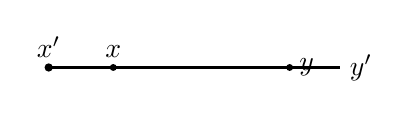
\begin{tikzpicture}[x=1cm,y=1cm]
\draw[thick](0,0)--(3.7,0);
\fill (0,0) circle (1.5pt) node[above]{$x'$};
\fill (.82,0) circle (1.25pt) node[above]{$x$};
\fill (3.06,0) circle (1.25pt) node[right]{$y$};
\node[right] at (3.7,0){$y'$};
\end{tikzpicture}}
) alors $y\in F$. On peut l'exprimer aussi en disant que
tt intervalle ouvert $\subset C$ qui rencontre $F$ est contenu ds $F$.

% L10–13
\uline{Prop} Toute facette de $C$ est convexe, \inserted{(non vide)}. $C$ est \deleted{\unsure{l'}}réunion disjointe de ses facettes

Considérons la relation dans $C$
\[
 R(x,y):\quad(x=y)\ \text{\uline{ou}}\ (x\text{ ni }y\text{ n'est extrémité de }C\cap D_{xy})
\]
\inserted{i.e. $x,y\in$ un intervalle ouvert $\subset C$}
\figure{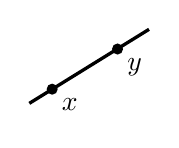
\begin{tikzpicture}[x=1cm,y=1cm]
\draw[very thick](0,0)--(1.52,.94);
\fill (.29,.18) circle (2pt) node[below right]{$x$};
\fill (1.12,.69) circle (2pt) node[below right]{$y$};
\end{tikzpicture}}

% L14–18
c'est une relation \deleted{\unsure{au moins}} d'équivalence : \unsure{réfl.} \inserted{\unsure{sym.}} évident ;
transitivité facile. Il est \unsure{clair|découle} aussi que
$\forall x\in C$, la classe de $x$ suivant
$R$ est l'unique facette qui contient $x$.

\figure{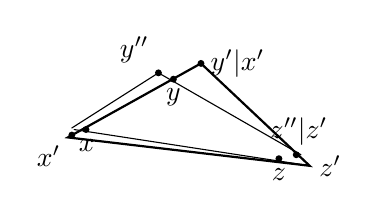
\begin{tikzpicture}[x=1cm,y=1cm,line cap=round]
\draw (.05,.12)--(1.15,.82)--(2.96,-.22);
\draw[thick](0,0)--(1.69,.94)--(3.07,-.36)--cycle;
\draw (.08,.10)--(3.07,-.36);
\foreach \x/\y in {.05/.03,.23/.10,1.15/.82,1.34/.74,1.69/.94,2.68/-.27,2.90/-.22}{\fill (\x,\y) circle(1.25pt);}
\node[below left] at (.03,.02){$x'$};
\node[below] at (.24,.1){$x$};
\node[above left] at (1.15,.82){$y''$};
\node[below] at (1.34,.74){$y$};
\node[right] at (1.69,.94){$\unsure{y'|x'}$};
\node[below] at (2.68,-.27){$z$};
\node[above] at (2.93,-.23){$\unsure{z''|z'}$};
\node[right] at (3.07,-.36){$z'$};
\end{tikzpicture}}

% L19–25
\uline{Prop} Soit $C$ un \uline{polyèdre} convexe (i.e. un ens
convexe qui est réunion finie d'enveloppes
\deleted{\unsure{f}} convexes de parties finies de l'espace affine
$E$)
% slanted
\margin{ou encore : int. \uline{finie} de demi-espaces fermés\ldots}
alors : \textcircled{1} l'ens des facettes est \uline{fini}. \textcircled{2} $\exists$ unique
facette maximale $\unsure{P|\mathcal P|\Phi}$, qui est aussi l'int de $C$ dans l'espace
affine engendré par $C$.

\textcircled{3} Pour tte facette $F$, $\overline F$ est une réunion de
facettes \deleted{\unsure{et on a} $\overline F\unsure{=|\supset} F'$ \unsure{(cf formule)|($F,F'$ facettes)} \unsure{ssi} $F=F'$}
\inserted{et, $F$ est l'unique facette $\subset\overline F$ de dimension max ($=\dim\overline F$)}

% L26–28 and lower left margin
\textcircled{4} et si celle ci est $d$, $\exists$ facette $\subset\overline F$ de dim $d-1$

% slanted
\margin{\textcircled{5} $C$ est l'env. convexe de la réunion \deleted{\unsure{des}} des facettes minimales ($=$ les pts extrémaux)}
% slanted
\margin{\textcircled{\unsure{6}} \deleted{\unsure{le}} \uline{bar.} de l'ens des pts extr. \unsure{ou des} facettes \unsure{minimales} \unsure{est au centre|est un centre|caractérise}}
\uline{Cor} Si $F,F'$ sont des facettes, $\overline F=\overline{F'}\Rightarrow F=F'$

Relation d'ordre entre facettes
